\documentclass[
	a4paper,
	10pt,
	unnumberedsections,
	twoside,
]{LTJournalArticle}

\usepackage{cleveref}
\usepackage{float}

\addbibresource{sample.bib}
\runninghead{WAL Protocol}
\footertext{\textit{What A Leak Protocol} (2024)}

\setcounter{page}{1}

\title{What A Leak Protocol\\ Rev 1.0}
\author{
	Yohan Boujon\textsuperscript{1}, Noel Jumin\textsuperscript{1}, \\ Clément Gauché\textsuperscript{1}, Robin Marin-Muller\textsuperscript{1}, Paul Jaulhiac\textsuperscript{1}, Cyril Vasseur\textsuperscript{1}
}

\date{\footnotesize\textsuperscript{\textbf{1}}INSA Toulouse, National Institute of Applied Sciences, Toulouse, France}

\renewcommand{\maketitlehookd}
{
	\begin{abstract}
        \noindent The \textbf{What A Leak} project aims to optimize its performance for data sharing via multiple nodes. These nodes need to communicate within a certain range, and because they can be many and far away from each other, a specific protocol has to be designed. There are two layers in this protocol, the first one being highlighted in Sec.\ref{sec:data-payload} will be the data processing layer, with multiple types that can be transferred and fields specific to the project's needs. The second layer will be discussed in Sec. \ref{sec:node-payload}, each nodes will be able to communicate with each other to transfer data over long range topology. These nodes need to identify the fastest path and will be helped by the main node. A cryptographic approach will be discussed in the Sub Sec. \ref{subsec:node-crypto} to help each node secure its data to the main gateway. There are some important constraints that we first need to talk about before entering into the depth of the tailored protocol. In Sec. \ref{sec:node-payload} every choices in term of timing, bandwidth, transmission power will be explained in details.
	\end{abstract}
}

\begin{document}

\maketitle
\section{Protocol main goal} \label{sec:constraints}
\subsection{Characteristics}
For around 2048 bytes every 30 seconds.
Bandwidth possible: 125/62.5 kHz -> spreading factor of SF10 for better Signal-to-Noise ratio, it will take 16-18 seconds to transfer all the data (will look into the detail of higher airtime so higher duty cycle). Using Coding Rate of 4/7 or 4/8 to increase error correction. Using 433.92 MHz for complex scenarios and less prone to error transmission.
\subsection{Node discovery and topology}
Spanning tree algorithm, topology will be stored in the main gateway.

\section{Header and Type}
\subsection{Addressing each Node}
ESP-32 are equipped with a Wi-Fi chip, whereas it has a Wi-Fi antenna or not, its MAC Address is globally unique accross all devices. \textit{Espressif} has the following identifier: \textbf{\textit{18:8B:0E}}, the other 6 bytes can be used as a unique identifier. This will be used in the first check to give each device a node ID that will be unique for the given topology.
\begin{figure}[H]
    \centering
    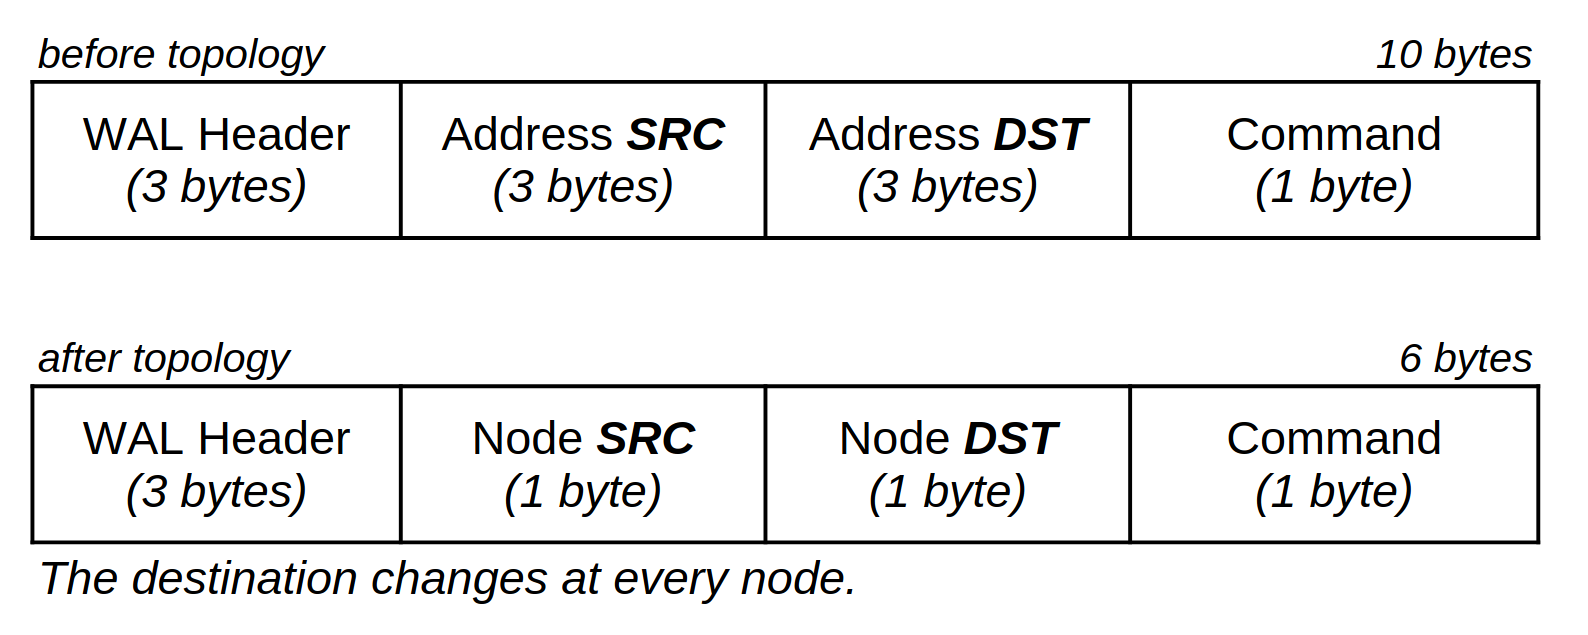
\includegraphics[width=0.9\linewidth]{img/wal_header.png}
    \caption{Start of the packet in two scenarios}
    \label{fig:wal_header}
\end{figure}
During the topology payload each node will communicate to the main node their MAC address on 3 bytes. Then an address on 1 byte will be sent back. This is made so that each packets will be smaller afterwards. As we can see on the picture above this does not change anything on the payload, only the final size. For the device to actually know which type of address the device has to read we have to look into the \textit{WAL header}.

\subsection{Header}
The start of each packet is strictly defined with 9 bits which are composed of "$wal$" in morse code. Then the version number on 7 bits each, for both major and minor version. If the version is not compatible or the 9 bits, which are equal to \textbf{\textit{0xd4}} are not recognized, the packet is instantly \textbf{rejected}.
\\
\\
1 bit is entirely dedicated to the type of address, either on 3 bytes (MAC based address), or 1 byte (Node ID given by the gateway). It can be described as the following:
\begin{figure}[H]
    \centering
    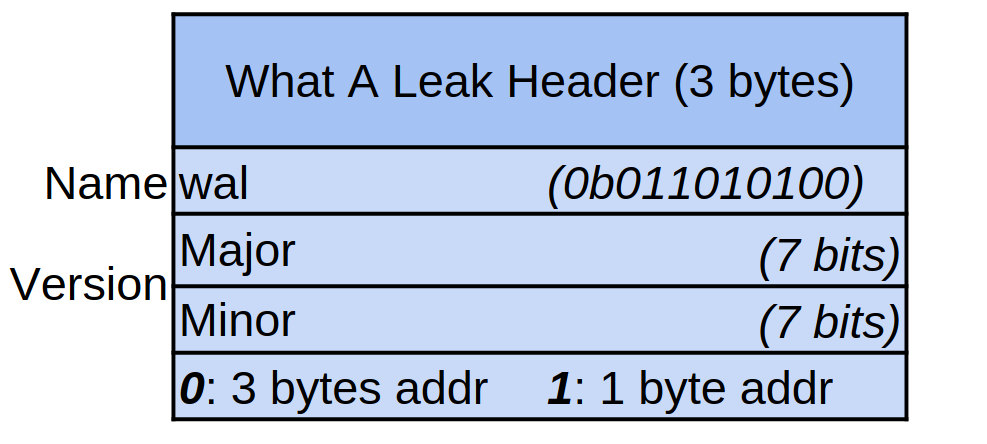
\includegraphics[width=0.9\linewidth]{img/wal_header_bits.png}
    \caption{Bits of the header}
    \label{fig:header_bits}
\end{figure}
\subsection{Command payload}
After checking if the packet has a correct header and if the data that is gathered is destinated to the correct device, a final check has to be done which is the command payload. This defines how the data should like like afterwards. It is entirely contained in 1 byte with the following bits:
\begin{figure}[H]
    \centering
    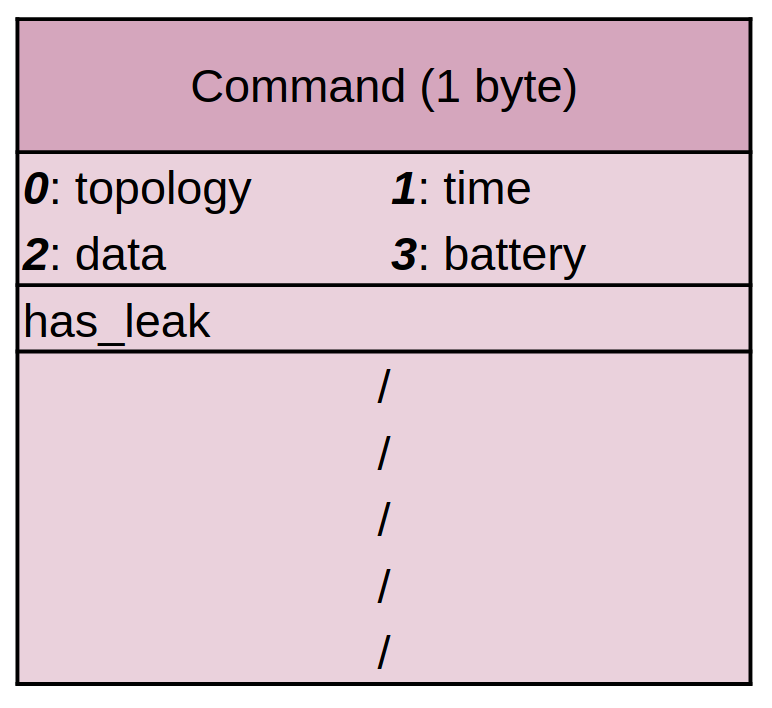
\includegraphics[width=0.6\linewidth]{img/command_bits.png}
    \caption{Bits of the command}
    \label{fig:command_bits}
\end{figure}
As we can see there are 4 types of command that can be sent by each device for now. It is stored in 4 bits, which can go up to 15 different commands that are yet to be defined (user-based could be applied here). After these command bytes we can have various data. One bit is dedicated to the \textit{has\_leak} derivative which is a verdict sent by the node's internal AI and FFT\footnote{\textbf{FFT}: Fast Fourier Transform} calculus.

\section{Topology payload}\label{sec:topology-payload}
Each node on the network need to gather a unique \textit{Node ID} as well as its underlying RSSI\footnote{\textbf{RSSI}: Received Signal Strength Indicator}. There could be multiple nodes that are close to the source device: by this mean, it can send multiple node with multiple level of signal strengths. This is how the payload can be described:
\begin{figure}[H]
    \centering
    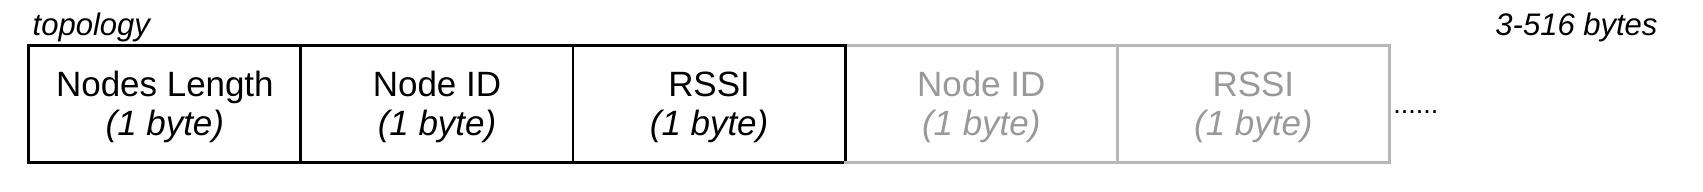
\includegraphics[width=1\linewidth]{img/topology.png}
    \caption{Topology Payload}
    \label{fig:topology}
\end{figure}

\section{Time payload}\label{sec:time-payload}
The internal RTC\footnote{\textbf{RTC}: Real-Time Clock} of each node may not be synchronize properly. With this payload, a ping-pong can be established between the closest device possible, calculating the possible drift. After testing with 10 exchanges, the EPOCH can be given on 8 bytes. The device has to add its delay and this way synchronize completely with the main gate. It has not been tested yet and may be fully precise, however, the time difference could be so minimal that it does not interfer with the FFT.
\begin{figure}[H]
    \centering
    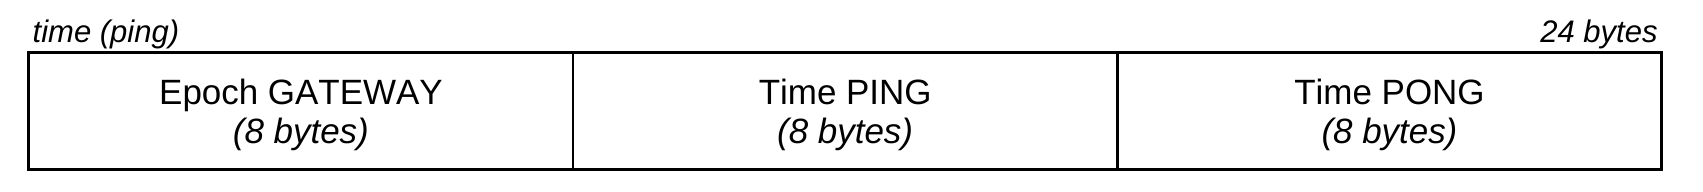
\includegraphics[width=1\linewidth]{img/time.png}
    \caption{Time Payload}
    \label{fig:time}
\end{figure}

\section{Data payload} \label{sec:data-payload}
Once everything is setup, it is now the time to send data. A data payload can have multiple types in itself, this is why there is 2 bytes header with the type (5-bits) and the size (13-bits). The 4 first bits are indicator of either 8,16,32 or 64 bits integers or a floating value (on 32-bits), a final 5th bit determine the signess of the underlying data.
\begin{figure}[H]
    \centering
    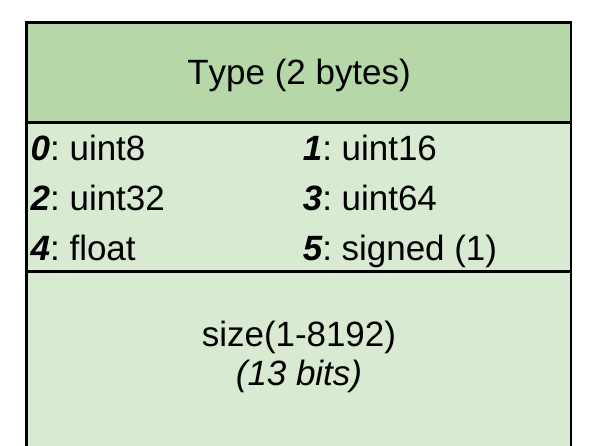
\includegraphics[width=0.6\linewidth]{img/type_bits.png}
    \caption{Type bits in Data Payload}
    \label{fig:type-bits}
\end{figure}

The data can then be delivered on \textit{8192 bytes maximum}.

\begin{figure}[H]
    \centering
    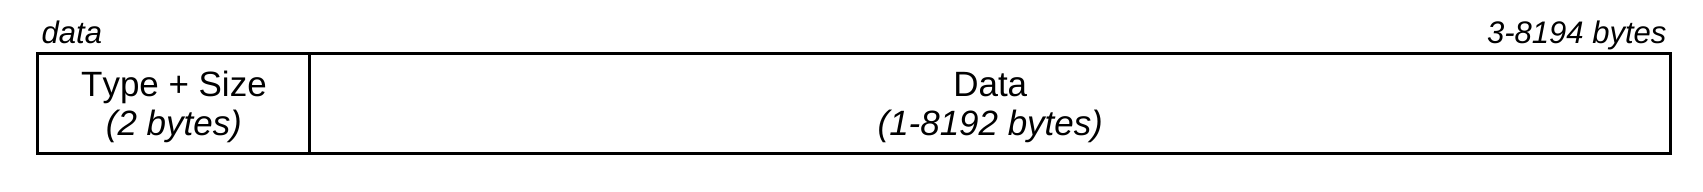
\includegraphics[width=1\linewidth]{img/data.png}
    \caption{Data Payload}
    \label{fig:data}
\end{figure}

\section{Battery payload} \label{sec:battery-payload}
Sometimes, we need to check the battery level of each node, a simple value on 1 byte can be send with the same logic as the topology payload seen in Sec.\ref{sec:topology-payload}.
\begin{figure}[H]
    \centering
    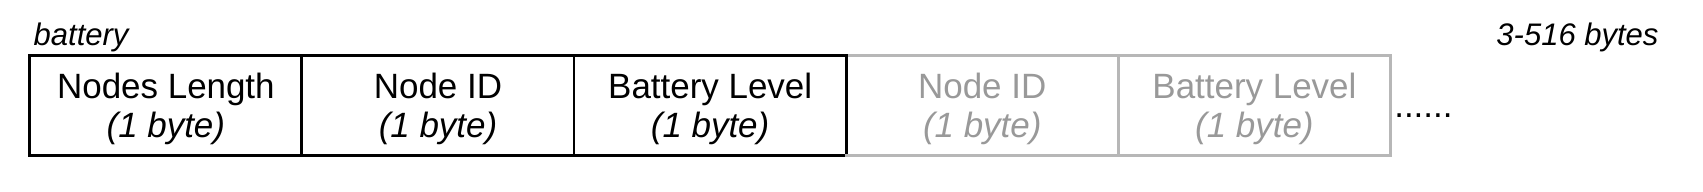
\includegraphics[width=1\linewidth]{img/battery.png}
    \caption{Battery Payload}
    \label{fig:battery}
\end{figure}

\section{Cryptography between node} \label{subsec:node-crypto}
Private key and public key from main gateway. Topology fixed or dynamic.

\section{Conclusion}

\nocite{*}
\printbibliography
\end{document}
